\begin{frame}{About JUnit}
	\begin{columns}[c]
		\begin{column}{5cm}\centering
			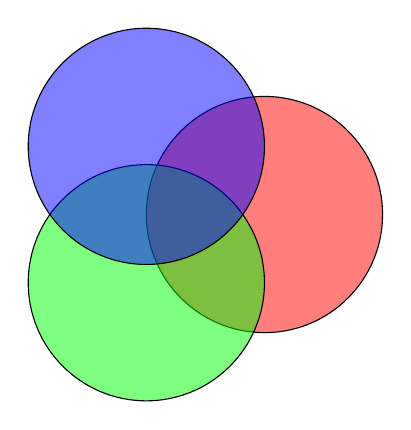
\begin{tikzpicture}
				\begin{scope}[fill opacity=.5]
					\filldraw[fill=red]   (0:1cm) circle (15mm);
					\filldraw[fill=green] (-120:1cm) circle (15mm);
					\filldraw[fill=blue]  (120:1cm) circle (15mm);
				\end{scope}
			\end{tikzpicture}
		\end{column}
		\begin{column}{5cm}
			\begin{block}{Kent Beck:}
				A programmer-oriented testing framework for Java.
			\end{block}
			\begin{block}{David Saff:}
				JUnit is the intersection of all possible useful Java test frameworks, not their union.
			\end{block}
			\vskip+1em
			Not only for Unit Tests!
		\end{column}
	\end{columns}
\end{frame}

\begin{frame}{A presentation about JUnit?}
	\begin{itemize}[<+->]
		\item Every Java developer knows JUnit.
		\item Really?
		\item Everyone thinks he knows JUnit.
		\item I thought so, too.
		\item However, a lot has happended since release 4.0!
	\end{itemize}
\end{frame}

\begin{frame}{New Features since 4.0}
\begin{center}
\begin{tikzpicture}[scale=0.9,transform shape]
  \path[every concept/.append style={font=\Large},level 1 concept/.append style={sibling angle=90,level distance=50mm},mindmap,concept color=gray,text=white]
    node[concept] {JUnit 4.8.2}
    child[grow=155,concept color=green!80]  { node[concept] {Matchers} }
    child[grow=205,concept color=blue!80]   { node[concept] {Theories} }
    child[grow=25,concept color=red!80]     { node[concept] {Rules} }
    child[grow=-25,concept color=orange!80] { node[concept] {Categories} };
\end{tikzpicture}
\end{center}
\end{frame}



{
\date{René Magritte, Untitled}
\usebackgroundtemplate{\includegraphics[width=\paperwidth,height=\paperheight]{img/matchers/part.jpg}}
\part{Matchers}
}

\begin{frame}[fragile]{New Assertion: \texttt{assertThat(\dots)}}
    \begin{itemize}
        \item New \texttt{Assert} methods:
    \begin{lstlisting}
<T> void assertThat(T actual, Matcher<T> matcher)
<T> void assertThat(String reason, T actual, Matcher<T> matcher)
\end{lstlisting}
        \item Parameters:
        \begin{description}[matcher]
            \item[reason]  description displayed when assertion fails (optional)
            \item[actual]  actual value
            \item[matcher] Hamcrest matcher that checks the actual value
        \end{description}
    \end{itemize}
\end{frame}

\begin{frame}[fragile]{Increased Readability}
    \only<1>{\javainputlisting[firstline=6]{hamcrest}{BetterReadability}}
    \only<2|handout:0>{\javainputlisting[firstline=6,emph={withoutMatchers,assertEquals}]{hamcrest}{BetterReadability}}
    \only<3|handout:0>{\javainputlisting[firstline=6,emph={withMatchers,assertThat}]{hamcrest}{BetterReadability}}
    \only<4|handout:0>{\javainputlisting[firstline=6,emph={is}]{hamcrest}{BetterReadability}}
    \begin{itemize}
        \item No more guessing about order of arguments
        \item Often more readable than traditional assertions
    \end{itemize}
\end{frame}

\begin{frame}[fragile]{Combining Matchers}
	Matchers are easily combined:
	\javainputlisting[firstline=20,lastline=21,tabsize=1]{hamcrest}{WithMatchers}
\end{frame}

\begin{frame}[fragile]{Expressive Failure Messages}
    \begin{block}{Traditional assertions without description}
\javainputlisting[firstline=10,lastline=10,tabsize=1]{hamcrest}{WithoutMatchers}
Result:
\begin{lstlisting}
AssertionError: at de.andrena.junit...
\end{lstlisting}
    \end{block}	
\pause
    \begin{block}{New assertion with matcher}
\javainputlisting[firstline=16,lastline=16,tabsize=1]{hamcrest}{WithMatchers}
Result:
\begin{lstlisting}
AssertionError:
Expected: not a collection containing <2>
     got: <[1, 2, 3]>
\end{lstlisting}
    \end{block}
\end{frame}

\begin{frame}{Predefined Matchers}
    \begin{itemize}
        \item Numerous predefined matchers:
        \begin{description}[Collections]
            \item[Core] \texttt{is}, \texttt{not}, \texttt{allOf}, \texttt{anyOf}, \texttt{nullValue}, \dots
            \item[Strings] \texttt{containsString}, \texttt{startsWith}, \texttt{endsWith}, \dots
            \item[Collections] \texttt{hasItem}, \texttt{hasItems}, \texttt{isIn}, \texttt{empty}, \texttt{hasSize}, \dots
        \end{description}
        \item JUnit includes only a small fraction:
        \begin{itemize}
            \item org.hamcrest.CoreMatchers
            \item org.junit.matchers.JUnitMatchers
        \end{itemize}
        \item Hamcrest offers additional matchers (\texttt{hamcrest-all.jar}).
        \item<alert@2> In addition, you can write your own matchers.
    \end{itemize}
\end{frame}

\begin{frame}{A Custom Matcher}{Implementation}
	\only<1>{\javainputlisting[firstline=9]{hamcrest}{IsEmptyCollection}}
	\only<2|handout:0>{\javainputlisting[firstline=9,emph={@Override,TypeSafeMatcher,matchesSafely,describeTo}]{hamcrest}{IsEmptyCollection}}
	\only<3|handout:0>{\javainputlisting[firstline=9,emph={@Factory, empty}]{hamcrest}{IsEmptyCollection}}
\end{frame}

\begin{frame}{A Custom Matcher}{Usage}
	\javainputlisting[firstline=9]{hamcrest}{CollectionMatchersTest}
\end{frame}

\begin{frame}{Many Matchers -- Many Classes}
	\begin{block}{Problem}
		\begin{itemize}
			\item Lots of matcher classes with static methods we would like to import
			\item Requires manual setup of preferences in IDE
			\item \dots for all developers!
		\end{itemize}
	\end{block}
	\begin{block}{Solution}
		Generate your own matcher library
	\end{block}
\end{frame}

\begin{frame}[fragile]{Generating a Custom Matcher Library}
	\begin{enumerate}
		\item Configuration in XML
			\lstinputlisting[language=XML,firstline=2]{java/EffectiveJUnit/src/de/andrena/junit/hamcrest/matchers.xml}
		\item Run \texttt{org.hamcrest.generator.config.XmlConfigurator}
		\item Combines all \texttt{@Factory} methods into a single generated class:
			\javainputlisting[firstline=7]{hamcrest}{Matchers}
	\end{enumerate}
\end{frame}

\begin{frame}[fragile]{Summary: Matchers}
	\begin{itemize}
		\item Assertions can often be expressed more elegantly
		\item Old assertion methods are still clearer sometimes
	\end{itemize}
	\begin{block}{Problem}
		Java type system often gets in one's way
		\begin{itemize}
			\item Requires boxing for primitive types \begin{lstlisting}
assertThat(1 + 1, is(2))
\end{lstlisting}
			\item Insufficient type inference \begin{lstlisting}
assertThat(new TreeSet<String>(), Matchers.<String>empty());
\end{lstlisting}
		\end{itemize}
	\end{block}
\end{frame}

{
\date{Wassily Kandinsky, Composition VIII}
\usebackgroundtemplate{\includegraphics[width=\paperwidth,height=\paperheight]{img/theories/part.jpg}}
\part{Theories}
}

\begin{frame}[fragile]{Parameterized Tests}
	\begin{itemize}
		\item \texttt{Parameterized} test runner included since JUnit 4.0
		\item Allows to supply parameters to test class constructors
		\item Arguments are defined in a public, static method
			\begin{itemize}
				\item \texttt{@Parameters} annotation
				\item Return type: \verb|List<Object[]>|
			\end{itemize}
		\item The runner creates an instance of the test class for each pair of test method and argument definition and executes the test. 
		\item Useful when testing a calculation with a large number of input values.
	\end{itemize}
\end{frame}

\begin{frame}{Parameterized Tests}{Example: Fibonacci Numbers}
	\only<1>{\javainputlisting[firstline=11]{fibonacci}{FibonacciParameterizedTest}}
	\only<2|handout:0>{\javainputlisting[firstline=11,emph={input, expected}]{fibonacci}{FibonacciParameterizedTest}}
	\only<3|handout:0>{\javainputlisting[firstline=11,emph={@Parameters,data}]{fibonacci}{FibonacciParameterizedTest}}
\end{frame}

\begin{frame}{Theories}
	\begin{itemize}
		\item Introduced in release 4.4
		\item Parameterized test method with preconditions (assumptions)
			\begin{itemize}
				\item \texttt{assumeThat()}
				\item \texttt{assumeTrue()}
				\item \texttt{assumeNotNull()}
			\end{itemize}
		\item \texttt{@Theory} instead of \texttt{@Test}
		\item Input for test methods via \texttt{@DataPoint}(\texttt{s}) annotation
	\end{itemize}
\end{frame}

\begin{frame}{Theories}{Example: Fibonacci Numbers}
	\only<1>{\javainputlisting[firstline=9]{fibonacci}{FibonacciTheories}}
	\only<2|handout:0>{\javainputlisting[firstline=9,emph={@Theory}]{fibonacci}{FibonacciTheories}}
	\only<3|handout:0>{\javainputlisting[firstline=9,emph={n}]{fibonacci}{FibonacciTheories}}
	\only<4|handout:0>{\javainputlisting[firstline=9,emph={assumeTrue}]{fibonacci}{FibonacciTheories}}
	\only<5|handout:0>{\javainputlisting[firstline=9,emph={@DataPoints,VALUES}]{fibonacci}{FibonacciTheories}}
	\only<6|handout:0>{\javainputlisting[firstline=9,emph={seeds}]{fibonacci}{FibonacciTheories}}
	\only<7|handout:0>{\javainputlisting[firstline=9,emph={recurrence}]{fibonacci}{FibonacciTheories}}
\end{frame}

\begin{frame}{Theories}{Example: \texttt{@DataPoints} of different types}
	\only<1>{\javainputlisting[firstline=9]{theories}{DifferentDataPoints}}
	\only<2|handout:0>{\javainputlisting[firstline=9,emph={@DataPoints,NUMBERS}]{theories}{DifferentDataPoints}}
	\only<3|handout:0>{\javainputlisting[firstline=9,emph={@DataPoint,A,B}]{theories}{DifferentDataPoints}}
	\only<4|handout:0>{\javainputlisting[firstline=9,emph={int,number,NUMBERS}]{theories}{DifferentDataPoints}}
	\only<5|handout:0>{\javainputlisting[firstline=9,emph={String,string,A,B}]{theories}{DifferentDataPoints}}
\end{frame}

\begin{frame}{Parameterized Tests vs. Theories}
	\begin{itemize}
		\item \texttt{@DataPoint} definition is more flexible
			\begin{itemize}
				\item Constants oder methods
				\item Any number of datapoints
				\item Different types
			\end{itemize}
		\item Test \emph{methods} are parameterized
			\begin{itemize}
				\item No boilerplate code (Constructor + instance variables)
				\item Different types of parameters possible
			\end{itemize}
		\item \texttt{Theories} can do everything \texttt{Parameterized} tests can, but more!
	\end{itemize}
\end{frame}

\begin{frame}{Traditional Tests vs. Theories}
	\begin{itemize}
		\item Traditional tests use examples:
			\begin{itemize}
				\item Validation of behaviour under selected inputs
				\item Examples ought to be characteristic (hopefully)
			\end{itemize}
		\item A theory generalizes a set of tests:
			\begin{itemize}
				\item precondition is made explicit
				\item assertions apply for all inputs that satisfy preconditions
			\end{itemize}
	\end{itemize}
\end{frame}


{
\date{René Magritte, Golconda}
\usebackgroundtemplate{\includegraphics[width=\paperwidth,height=\paperheight]{img/rules/part.jpg}}
\part{Rules}
}

\begin{frame}<1-2>[label=ruledef]{What is a Rule?}
	Extension mechanism for execution of test methods
	\begin{block}{Examples:}
		\begin{itemize}
			\item<alert@2> Execute code before/after every test method
			\item<alert@3> Handle failed tests
			\item Check additonal criteria after every test
			\item \dots
		\end{itemize}
	\end{block}
\end{frame}

\begin{frame}{Example: TemporaryFolder}{Without Rules}
	\only<1>{\javainputlisting[firstline=9,lastline=27]{rules}{TemporaryFolderWithoutRule}}
	\only<2|handout:0>{\javainputlisting[firstline=9,lastline=27,emph={@Before,@After,folder}]{rules}{TemporaryFolderWithoutRule}}
\end{frame}

\begin{frame}{Example: TemporaryFolder}{With Rules}
	\only<1>{\javainputlisting[firstline=9]{rules}{TemporaryFolderWithRule}}
	\only<2|handout:0>{\javainputlisting[firstline=9,emph={@Rule,folder}]{rules}{TemporaryFolderWithRule}}
\end{frame}

\againframe<3>{ruledef}

\begin{frame}{Example: ExpectedException}{Without Rules}
	\only<1>{\javainputlisting[firstline=7]{rules}{ExpectedExceptionWithoutRule}}
	\only<2|handout:0>{\javainputlisting[firstline=7,emph={expected}]{rules}{ExpectedExceptionWithoutRule}}
\end{frame}

\begin{frame}{Example: ExpectedException}{With Rules}
	\only<1>{\javainputlisting[firstline=7]{rules}{ExpectedExceptionWithRule}}
	\only<2|handout:0>{\javainputlisting[firstline=7,emph={@Rule,thrown}]{rules}{ExpectedExceptionWithRule}}
\end{frame}

\begin{frame}{Other Predefinded Rules}
	\begin{block}{ErrorCollector}
		Collects failing assertions and causes the test to fail with an aggregated list of failures at the end.
	\end{block}
	\begin{block}{TestName}
		Provides access to the name of the currently executing test method.
	\end{block}
	\begin{block}{Timeout}
		Applies the same timeout to all test methods in the test class.
	\end{block}
\end{frame}

\begin{frame}{Write Your Own Rules!}
	\includegraphics<1|handout:0>[width=\textwidth]{img/rules/basisKlassen.jpg}
	\includegraphics<2>[width=\textwidth]{img/rules/basisKlassenMitTemporaryFolder.jpg}
\end{frame}

\begin{frame}{Custom Rule}{Implementation}
	\only<1>{\javainputlisting[firstline=5]{rules}{SystemProperty}}
	\only<2|handout:0>{\javainputlisting[firstline=5,emph={@Override,before,after,ExternalResource}]{rules}{SystemProperty}}
\end{frame}

\begin{frame}{Custom Rule}{Usage}
	\only<1>{\javainputlisting[firstline=8]{rules}{SomeTestUsingSystemProperty}}
	\only<2|handout:0>{\javainputlisting[firstline=8,emph={@Rule,systemProperty}]{rules}{SomeTestUsingSystemProperty}}
\end{frame}

\begin{frame}{Advantages of Rules}
	\begin{block}{Reusable}
		Allow to encapsulate frequently used code.
	\end{block}
	\begin{block}{Composable}
		You can use any number of rules in one test class.
	\end{block}
	\begin{block}{Delegation over inheritance}
		Help to avoid test class hierarchies.
	\end{block}
	\begin{block}{Extendable}
		Writing your own rules is easy.
	\end{block}
\end{frame}

{
\date{Piet Mondrian, Composition with Gray and Light Brown}
\usebackgroundtemplate{\includegraphics[width=\paperwidth]{img/categories/part.jpg}}
\part{Categories}
}

\begin{frame}{Dividing Tests into Categories}
	\begin{itemize}
		\item Category is class or interface:
			\javainputlisting[firstline=3]{categories}{Slow}
		\item Only for one test:
			\javainputlisting[firstline=13,lastline=15,tabsize=1]{categories}{A}
		\item All tests in a test class:
			\javainputlisting[firstline=6]{categories}{B}
	\end{itemize}
\end{frame}

\begin{frame}{Executing All Tests in Certain Categories}
	\begin{itemize}
		\item Conventional test suite:
			\javainputlisting[firstline=7]{categories}{AllTests}
		\item All tests in category \texttt{Slow}:
			\javainputlisting[firstline=7]{categories}{AllSlowTests}
		\item All other tests:
			\javainputlisting[firstline=7]{categories}{AllFastTests}
	\end{itemize}
\end{frame}

{
\date{Quint Buchholz, Mann auf einer Leiter}
\usebackgroundtemplate{\includegraphics[width=\paperwidth,height=\paperheight]{img/summary/part.jpg}}
\part{What's next?}
}

\begin{frame}{What's next?}
	\begin{itemize}
		\item Updating to more recent JUnit version is easy
		\item Old tests will still run
		\item New tests will benefit from new features
		\item Old tests can be simplified little by little
		\item<alert@2> Try it out!
	\end{itemize}
\end{frame}

\begin{frame}{Try it out!}

	{%\Large
	\url{http://www.junit.org/}\par
	\url{https://github.com/marcphilipp/junit-4x-presentation}\par}\vskip+1em

	\begin{beamercolorbox}[sep=1em]{blockbackground} 
		In theory, there is no difference between theory and practice.\\
		But, in practice, there is.\par\vskip-.5em
		\hfill\scriptsize Jan L. A. van de Snepscheut/Yogi Berra
	\end{beamercolorbox}\vskip+.5em

	{\centering\Huge
	Thank you!\par}\vskip+1em

	\begin{description}[Twitter]
		\item[Mail]    \href{mailto:marc@andrena.de}{\texttt{marc@andrena.de}}
		\item[Twitter] \href{http://twitter.com/marcphilipp}{\texttt{@marcphilipp}}
		\item[Blog]    \url{http://marcphilipp.tumblr.com/}
	\end{description}
\end{frame}

